\documentclass{article}

% Language setting
% Replace `english' with e.g. `spanish' to change the document language
\usepackage[en
glish]{babel}

% Custom packages
\usepackage{color,soul} % For highlighting text
\usepackage{float} % For controlling figure placement ([H] option)
\usepackage{amsmath}
\usepackage{amssymb} % For mathematical symbols such as \lessgtr
\DeclareMathOperator*{\argmax}{arg\,max}
\DeclareMathOperator*{\argmin}{arg\,min}

% Set page size and margins
% Replace `letterpaper' with `a4paper' for UK/EU standard size
\usepackage[letterpaper,top=2cm,bottom=2cm,left=3cm,right=3cm,marginparwidth=1.75cm]{geometry}

% Useful packages
\usepackage{graphicx}
\usepackage[colorlinks=true, allcolors=blue]{hyperref}

\definecolor{mulberry}{rgb}{0.77, 0.29, 0.55}
\newcommand{\dm}[1]{{\color{mulberry} #1}}

\newcommand{\mi}{\mathrm{i}}

\title{Analyse statistique des distributions de sortie du Kernel-Nulling pour la détection à haut contraste d'exoplanètes dans les configurations VLTI et LIFE}

\author{Vincent Foriel,
        David Mary,
        Frantz Martinache
       }

\begin{document}

\maketitle

\begin{abstract}
L'interférométrie à annulation par noyau (Kernel-Nulling) représente une approche prometteuse pour la détection directe d'exoplanètes. Cette technique génère des distributions d'intensité caractéristiques selon la présence ou l'absence d'un compagnon planétaire. L'analyse statistique de ces distributions est essentielle pour une détection robuste de planètes. Nous développons et comparons plusieurs tests statistiques pour discriminer efficacement entre les hypothèses $\mathcal{H}_0$ (étoile seule) et $\mathcal{H}_1$ (système étoile-planète). Nous analysons les performances de différentes statistiques de test afin d'évaluer la pertinence de chacun d'eux en fonction de la nature des données à disposition. Nous effectuons des simulations numériques pour trois scenarios instrumentaux : les configurations VLTI au sol et celle de LIFE dans l'espace ainsi qu'un scénario fictif consistant à placer le VLTI dans l'espace afin d'isoler les pertes de performance causées par l'atmosphère. Pour chaque scénario, nous générons des jeux de données sous les deux hypothèses $\mathcal{H}_0$ et $\mathcal{H}_1$, en tenant compte des paramètres instrumentaux spécifiques et des niveaux de bruit. Nous évaluons les performances des tests en utilisant les courbes ROC et l'analyse des valeurs P. \hl{Ajouter les résultats}. Cette analyse statistique, actuellement appliquée à des données simulées, ouvre la voie à une détection robuste d'exoplanètes à haut contraste utilisant l'interférométrie à annulation par noyau.
\end{abstract}

\dm{OK résumé de mes coms détailles ci-dessous : le plus gros boulot à faire pour l'itération suivante c'est : \\
- en intro : biblio : recenser, comparer, contraster pour mettre en évidence l'originalité du papier\\
- en intro : justification de l'intérêt scientifique du papier (/exoplanètes, VLTI, LIFE) et de son scope (portée attendu des simus ?) \\
- Sec. 2 étude statistique plus poussée des différents régimes, types de distribution, influence des paramètres, classement et présentation des résultats pour justifier la section d'après (les tests mis en opuvre)\\
- Sec. 3 : La formalisation rigoureuse des tests, classement, formules analytiques \\
- Sec. 4 : Etude comparative des performances dans les résultats }

%==============================================================================
\section{Introduction}
%==============================================================================

L'imagerie directe d'exoplanètes demeure l'un des défis majeurs de l'astronomie moderne, nécessitant des techniques capables de surmonter les contraintes de contraste (au-delà de $10^{-8}$ pour permettre la détection d'exo-Terres) et les exigences de séparation angulaire (de l'ordre de milli-arcseconde). L'interférométrie à annulation, initialement proposée par \cite{Bracewell1979}, utilise l'interférence destructive pour supprimer la source sur l'axe (lumière stellaire) tout en préservant celles hors axe (signaux planétaires), répondant ainsi aux défis de résolution angulaire et de contraste.

Le Kernel-Nulling (\cite{Martinache2018}) améliore cette approche en se concentrant sur la différence entre des paires de combinaisons  symétriques de faisceaux qui sont robustes aux aberrations de phase du premier ordre (\cite{Martinache2018}). En raison de différentes sources de perturbations, la sortie de l'opération d'annulation - ainsi que l'opération de Kernel-Nulling - est une distribution statistique d'intensités. Cette distribution est influencée par divers paramètres instrumentaux tels que les erreurs de cophasage en entrée, les erreurs d'amplitude, le nombre de trames, le fond de ciel ou même d'autres sources de lumière indésirables comme, par exemple, étoiles d'arrière-plan (\cite{Hanot2011}, \cite{Cvetojevic2022}). La présence d'un compagnon induit une erreur de cophasage systématique qui ne peut être approximée par une perturbation du premier ordre, conduisant à un décalage global dans les distributions de sortie du Kernel-Null. Cela résulte en des distributions statistiques distinctes pour la sortie du kernel-null selon qu'un compagnon soit présent ou non (voir Fig. \ref{fig:distribution}). Dans des scénarios réalistes, le décalage induit par la présence du compagnon est petit comparé à la dispersion due aux différentes sources de perturbation, rendant les distributions $\mathcal{H}_0$ et $\mathcal{H}_1$ difficiles à distinguer. Le nombre de trames utilisé dans la simulation affecte également l'étalement et la lissité des distributions. Une analyse détaillée de l'influence de ces paramètres et des familles de distributions résultantes est fournie en Sec. \ref{sec:distribution_analysis}. Cependant, ces distributions ne suivent pas les lois de probabilité standard, et leur forme analytique est inconnue a priori. Cela rend le problème de discrimination difficile, en particulier lorsque le contraste du compagnon est élevé et que les distributions se chevauchent significativement.

L'analyse de ces distributions nécessite donc des outils statistiques appropriés pour discriminer efficacement entre les deux hypothèses : $\mathcal{H}_0$ (étoile seule) et $\mathcal{H}_1$ (système étoile-planète). Dans ce travail, nous développons et comparons plusieurs tests statistiques pour optimiser la détection d'exoplanètes utilisant le Kernel-Nulling.

\dm{Il manque :\\
- Une biblio minutieuse de ce pb : mettre en évidence des différence entre des distributions dans un contexte exoplanètes, et plus généralement astro, ça existe où ? Comment les gens font ? Qu'est-ce que tu prends d'eux et qu'est ce que tu vas apporter de nouveau ? Quelles différences entre les problématiques connexes que tu as trouvées et la tienne ? Expliquer points communs et différences.\\
- Justification de l'intérêt de ce papier par rapport aux instruments visés / VLTI et LIFE. Faire un topo sur VLTI et lIFE par rapport à la détection d'exoplanètes. Puis décrire comment l'approche kernel-nulling se compare aux autres approches de détection exoplanètes (pros/cons) ? Et enfin sur l'approche quel est le statut des méthodes prévues ? (en gros : on ne sait pas vraiment faire, ton papier est très important pour poser des algos. Mais attention contraster par rapport aux travaux de Hanot \& co que je t'ai fait suivre par mail; et il y en a probablement d'autres.)\\ 
- plan du papier}

\begin{figure}[H]
\centering
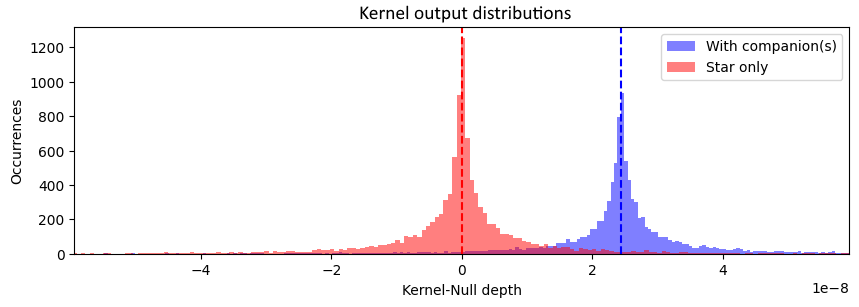
\includegraphics[width=\linewidth]{img/output_distribution.png}
\caption{Exemple de distributions de profondeur d'annulation par noyau pour les hypothèses $\mathcal{H}_0$ (étoile seule) et $\mathcal{H}_1$ (avec compagnon). Ce scénario d'exemple est fortement exagéré avec un compagnon qui a un faible contraste afin d'induire un décalage significatif de la distribution. En pratique, les deux distributions sont généralement beaucoup plus proches et difficiles à distinguer.\dm{Cf texte; aussi prends l'habitude d'être ultra-spécifique, c'est un papier scientifique. Là tu es bcp trop vague : "low contrast" (c'est quoi low ?) "much closer" (=?..)}.}
\label{fig:distribution}
\end{figure}



%==============================================================================
\section{Méthodologie}
%==============================================================================



%------------------------------------------------------------------------------
\subsection{Génération de données}

Dans cette étude, nous considérons trois scénarios instrumentaux correspondent à des configurations réalistes d'interféromètres dédiés à la détection d'exoplanètes, chacune avec ses propres contraintes technologiques et performances attendues.

\textbf{Le Very Large Telescope Interferometer (VLTI)} représente l'état actuel de l'art en interférométrie au sol. Cet instrument combine la lumière de quatre télescopes unitaires (UT) de 8 mètres de diamètre chacun, disposés en configuration irrégulière avec une ligne de base maximale de 130 mètres. Cette configuration permet d'atteindre une résolution angulaire théorique de l'ordre de 1 milli-arcseconde à $1.55\mu$m, longueur d'onde optimale pour l'observation dans la bande H du proche infrarouge. Cependant, les conditions atmosphériques terrestres introduisent des perturbations de phase significatives : malgré les systèmes d'optique adaptative et de correction de cophasage en temps réel, l'erreur de cophasage résiduelle demeure de l'ordre de 100 nm RMS. Cette valeur, bien que représentant une performance remarquable pour un instrument au sol, constitue néanmoins une limitation fondamentale pour la détection d'exoplanètes à très haut contraste, où la stabilité de phase doit être maintenue à des niveaux extrêmes sur des temps d'intégration longs.

\textbf{La mission spatiale LIFE (Large Interferometer For Exoplanets)} incarne l'avenir de l'interférométrie dédiée à la détection d'exoplanètes. Cette mission prévoit le déploiement en orbite de quatre télescopes de 2 mètres de diamètre arrangés en formation rectangulaire avec une ligne de base pouvant atteindre 600 mètres. L'environnement spatial offre des avantages décisifs : l'absence d'atmosphère élimine les turbulences et permet un contrôle de phase d'une précision inégalée, avec des erreurs de cophasage réduites à 1 nm RMS. Cette stabilité exceptionnelle, couplée à la longueur d'onde d'observation de $4\mu$m dans l'infrarouge thermique, ouvre la voie à la détection directe d'exo-Terres et à la spectroscopie de leurs atmosphères pour la recherche de biosignatures.

\textbf{Le scénario SVLTI (Space VLTI)} constitue un cas d'étude théorique permettant d'isoler l'impact spécifique de l'atmosphère terrestre sur les performances de détection. En transposant la configuration exacte du VLTI (quatre télescopes de 8 mètres, disposition irrégulière, ligne de base de 130 mètres) dans l'environnement spatial, nous conservons la même longueur d'onde d'observation ($1.55\mu$m) tout en bénéficiant de la stabilité de cophasage spatiale (1 nm RMS). Cette configuration hybride permet une analyse comparative directe : en comparant les performances VLTI/SVLTI, nous quantifions précisément la dégradation causée par les perturbations atmosphériques, tandis que la comparaison SVLTI/LIFE révèle l'impact de l'architecture instrumentale (taille des télescopes, longueur d'onde, géométrie) sur l'efficacité de détection.

En résumé, nous avons donc :
\begin{table}[H]
\centering
\begin{tabular}{|l|c|c|c|}
\hline
\textbf{Paramètre} & \textbf{VLTI} & \textbf{LIFE} & \textbf{SVLTI} \\
\hline
Nombre de télescopes & 4 & 4 & 4 \\
Diamètre des télescopes & 8 m & 2 m & 8 \\
Configuration & Irrégulière & Régulière (rectangulaire) & Irrégulière \\
Ligne de base maximale & 130 m & 600 m & 130 \\
Environnement d'exploitation & Sol & Espace & Espace \\
Longueur d'onde & $1.55\mu$m & $4\mu$m & $1.55\mu$m \\
Erreur de cophasage (RMS) & 100 nm & 1 nm & 1 nm \\
\hline
\end{tabular}
\caption{Paramètres instrumentaux pour les trois scénarios considérés dans cette étude.}
\label{tab:scenarios}
\end{table}

Pour chacune des simulations réalisées, nous considérons une source primaire de magnitude zero (étoile type Vega) avec un compagnon hypothétique unique dont on fixe la position et le contraste. Ce travail s'intéressant aux limites théoriques atteignables en terme de capacité de détection, nous travaillons sous l'hypothèse d'une environnement thermiquement stable et d'une caméra idéale, c'est-à-dire sans bruit de lecture ni bruit de fond. Nous simulons des séries d'acquisitions de 1 seconde en intégrant les effets des erreurs de cophasage résiduelles (perturbations atmosphériques et différence de chemin optique intrasèque au système) et de bruit photonique. Pour chaque scénario, nous générons des jeux de données sous les deux hypothèses $\mathcal{H}_0$ (étoile seule) et $\mathcal{H}_1$ (système étoile-planète), en tenant compte des paramètres instrumentaux spécifiques et des niveaux de bruit pour chaque cas.



%------------------------------------------------------------------------------
\subsection{Tests statistiques et rapport de vraisemblance}

Pour discriminer entre les hypothèses $\mathcal{H}_0$ (étoile seule) et $\mathcal{H}_1$ (système étoile-planète), plusieurs statistiques de test sont utilisées dans nos simulations :

\begin{itemize}
    \item \textbf{Moyenne} : $T(u) = |\mathrm{mean}(u)|$
    \item \textbf{Médiane} : $T(u) = |\mathrm{median}(u)|$
    \item \textbf{Kolmogorov-Smirnov} : $T(u, v) = |D_{KS}(u, v)|$ où $D_{KS}$ est la statistique KS entre deux échantillons
    \item \textbf{Flattening} : $T(u) = \sum_i |u_i - \mathrm{median}(u)|$
\end{itemize}

Chaque test permet de quantifier la différence entre les distributions issues des deux hypothèses. Les performances sont évaluées via les courbes ROC et l'analyse des valeurs P.

Pour chaque scénario, des jeux de données sont générés sous les deux hypothèses $\mathcal{H}_0$ (étoile seule) et $\mathcal{H}_1$ (système étoile-planète), en tenant compte des paramètres instrumentaux spécifiques et des niveaux de bruit pour chaque cas. L'opération de Kernel-Nulling est supposée idéale.\dm{Je pense qu'il faut prévoir un appendice où tu résumes le principe de kernel-nulling pour que le lecteur te suive; qu'il comprenne ce que signifie faire une operaiton de kernel nulling en pratique, et lister tous les défauts qui font que ça ne peut pas être idéal. Il faut aussi différencier une operation de kernel null idéale et l'absence de bruit à la fin. Bien expliquer ce que capturent tes simulations et les fluctuations qui créent les distributions montrées en Fig. 1.}



%------------------------------------------------------------------------------
\subsection{Analyse des distributions}  \label{sec:distribution_analysis}

Avant de tenter de discriminer entre les hypothèses $\mathcal{H}_0$ et $\mathcal{H}_1$, il est essentiel d'étudier les distributions obtenues pour identifier les caractéristiques qui pourraient faciliter leur analyse. À cette fin, nous comparons les distributions simulées à différentes lois de probabilité conventionnelles, en observant notamment leur symétrie et leur forme générale.

Nous trouvons qu'aucune loi conventionnelle ne correspond parfaitement aux distributions observées. \dm{$<=$ Ca c'est une conclusion. Pour que cette phrase ait du poids, il faut présenter une analyse détaillée de ces distributions (comme le titre le suggère) : montrer comment les variations combinées de tous les paramètres importants mènent à des distributions différentes. Identifier et montrer tous les différents régimes de paramètres menant à des familles de distributions différentes. Lister aussi tous les pramètres qui vont entrer en compte dans les perfs de détections : contraste et position du compagnon, longueur d'onde donc, nombre de trames, puissance des erreurs de phase, D telescope,... tu peux faire une table. Une étude scientifique est vraiment une étude scientifique : on essaie d'être exhaustif dans l'analyse, et ensuite de faire une synthèse quantifiée et bien rangée qui reflète clairement tous les cas pour le lecteur. Le but est d'en faire un expert en lui donnant toutes les infos pour qu'ils le deviennent en lisant le papier, et puisse reproduire les résultats s'il le souhaite (c'est le propre de la démarche scientifique, éviter d'être juste déclaratif ce qui revient à proposer des arguments d'autorité; préférer systématiquement être aussi précis que possible et donner toutes les infos, ce qui revient à proposer des arguments d'expertise.} Parmi les lois testées, la distribution de Cauchy semble \dm{c'est faible et pas quantifié, et vu la fig.2 ça ne colle pas comme tu le dis} offrir un ajustement relativement satisfaisant (Fig. \ref{fig:fits}), bien que non parfait, en particulier sur les queues lorsque le nombre d'échantillons est élevé.

Cette observation guide le choix des tests statistiques à privilégier, en particulier ceux efficaces pour détecter des décalages dans les distributions symétriques.\dm{Justifier théoriquement et/ou empiriquement (via l'optique et le ssimus) si les distribution doivent être symétriques. Ajouter éveutellement des acquisitions de frames sur banc pour appuyer à un moment ces hypothèses. } De plus, cela suggère que l'ajustement de données en minimisant \dm{$<=$ data fitting of what ? Pas le fit de d'une distribution empirique par une autre en tout cas... on en discutera. } l'erreur quadratique moyenne (MSE) ne sera très probablement pas très efficace en raison des queues lourdes de la distribution. Au lieu de cela, nous devrions utiliser une fonction de coût dérivée de la loi de Cauchy, qui est plus robuste aux valeurs aberrantes :\dm{Non je pense que la fin de la section n'est pas bonne.}
\begin{equation}
    \text{Cost}(x, y) = \sum_i \log \left( 1 + \left( y_i - s(x_i )\right)^2 \right)
\end{equation}

\begin{figure}[H]
\centering
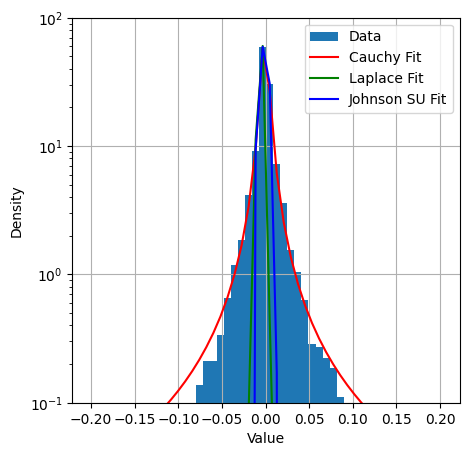
\includegraphics[width=6cm]{img/fits.png}
\caption{Ajustement des lois de probabilité conventionnelles aux distributions simulées. Le package Python Fitter a été utilisé pour effectuer l'ajustement de la plupart des lois usuelles. Cette figure montre l'ajustement des trois lois les plus pertinentes que le package a identifiées.}
\label{fig:fits}
\end{figure}



%------------------------------------------------------------------------------
\subsection{Tests statistiques implémentés}

\dm{Expliquer la démarche : vu le pb on a logiquement envie d'implémenter  des tests globaux qui mesurent un shift (et rejustifer que c'est juste un shift si c'est bien le cas.\\
- Puis dire qu'on peut aller plus loin : il est naturel de regarder des mesures plus globales entre les distributions et là tu pars sur  KS etc. Ajoute Anderson-Darling dans cette famille.\\
- Ensuite 1) présente tes notations (par ex, qu'est-ce que $x$ ? 2) rappelle précisément ce que tu appelles $\mathcal{H}_0$ et $\mathcal{H}_1$ en utilisant les quantitiés de  tes notations.\\
- Ensuite, pour chaque test, de façon systématique : 0) Donne la ref du/des papiers scientifiques où il a été décrit (pas une ref à une toolbox python; un bouquin tu peux, mais il faut aussi les refs originales \#démarche scientifique vérifiable etc) 1) explique l'intuition derrière 2) donne la stat de test (en utilisant les notations définies avant) 3) explique s'il y a une formule analytique pour décrire la stat de test sous $\mathcal{H}_0$ (explique aussi avant fe lister les tests  que l'intérêt d'une formule analytique est  que ça donne accès à une p-valeur sans avoir à faire des simus de Monte Carlo, et les pbs que posent le fait de devoir faire des MC (calcul mais surtout on doit pouvoir simuler les mêmes conditions de perturbations que les données !)). Par exemple, avec le Th Centrale limite, si les $x_i$ sont i.i.d (pas forcément gaussiens comme dans notre cas), la stat de test (2) est gaussienne de variance connue donc pour (2) ça devrait être bon.\\
- Dans les cas où une distribution est disponible, vérifier par simus et montrer que la distribution empirique correpond bien à la théorique.}

En présence d'un compagnon (hypothèse $\mathcal{H}_1$), la distribution de sortie du Kernel-Nulling est modifiée par rapport au cas de l'étoile seule (hypothèse $\mathcal{H}_0$) comme le montre la figure \ref{fig:distribution}.

Cette modification se manifeste principalement par un décalage de la distribution, bien que d'autres changements dans la forme de la distribution puissent également survenir. En fonction des conditions, il est par exemple possible de constater un applatissement de la distribution. Pour détecter efficacement la présence d'un compagnon, nous avons implémenté et évalué plusieurs tests statistiques, chacun étant sensible à différents aspects des distributions.

%~~~~~~~~~~~~~~~~~~~~~~~~~~~~~~~~~~~~~~~~~~~~~~~~~~~~~~~~~~~~~~~~~~~~~~~~~~~~~~
\subsubsection{Moyenne}

Le test le plus naturel a faire dans ces conditions consiste à comparer la moyenne à un seuil. Etant donné que la planète peut induire un décallage de la distribution dans les deux sens, on utilise la valeur absolue de la moyenne.

$$
D_{M} = \left|\frac{1}{N}\sum_{i=1}^N x_i \right| \stackrel{H_1}{\underset{H_0}{\gtrless}} \xi
$$

En effet, sous l'hypothèse $\mathcal{H}_0$, la moyenne devrait être proche de zéro, équivalent à la moyenne du bruit $\bar{n}$, tandis que sous $\mathcal{H}_1$, elle sera décalée en fonction du signal de la planète $S_p$ et de sa transmission $\alpha$ au sein du système.

$$
\begin{cases}
H_0 : D_M = |\bar{n}|\\
H_1 : D_M =  |\alpha S_p + \bar{n}|
\end{cases}
$$

En pratique, on constate que la moyenne est ici une statistique de test particulièrement peu fiable (figure \ref{fig:roc}). En effet, cette dernière est sensible aux valeurs extrêmes, or les distributions considérées ont des queues lourdes.

%~~~~~~~~~~~~~~~~~~~~~~~~~~~~~~~~~~~~~~~~~~~~~~~~~~~~~~~~~~~~~~~~~~~~~~~~~~~~~~
\subsubsection{Médiane}
Une autre statistique de test naturelle dans ce contexte est la médiane, qui est plus robuste aux valeurs extrêmes que la moyenne. La médiane est définie comme la valeur centrale d'un ensemble de données triées. Pour un ensemble de données $x_1, x_2, \ldots, x_N$ triées en ordre croissant, la médiane est alors la valeur de l'élément central si $N$ est impair, ou la moyenne des deux éléments centraux si $N$ est pair. Comme pour la moyenne, on utilise la valeur absolue de la médiane pour capturer les décalages dans les deux sens qu'on compare ensuite à un seuil.

$$
D_m = 
\begin{cases}
\left| x_{\frac{N+1}{2}} \right| & \text{if }N\text{ is odd} \\

\left| \frac{x_{\frac{N}{2}} + x_{\frac{N+1}{2}}}{2} \right|  & \text{if }N\text{ is even}
\end{cases}
\quad\stackrel{H_1}{\underset{H_0}{\gtrless}} \xi
$$

De façon très analogue, sous l'hypothèse $\mathcal{H}_0$, la médiane devrait être proche de zéro, équivalent à la médiane du bruit $\tilde{n}$, tandis que sous $\mathcal{H}_1$, elle sera décalée en fonction du signal de la planète $S_p$ et de sa transmission $\alpha$ au sein du système.

$$
\begin{cases}
H_0 : D_m = |\tilde{n}|\\
H_1 : D_m =  | \alpha S_p + \tilde{n} |
\end{cases}
$$

Surprenament, la médiane s'avère être une statistique de test très performante dans ce contexte (figure \ref{fig:roc}), surpassant bon nombre de tests plus sophistiqués comme ceux listés dans la section \ref{sec:other_tests}. Cependant, elle necessite un grand nombre d'échantillons pour être efficace, ce qui peut être un inconvénient dans des situations où le temps d'observation est limité.

%~~~~~~~~~~~~~~~~~~~~~~~~~~~~~~~~~~~~~~~~~~~~~~~~~~~~~~~~~~~~~~~~~~~~~~~~~~~~~~
\subsubsection{Kolmogorov-Smirnov}
\dm{Attention c'est le 2-sided KS}

Le test de Kolmogorov-Smirnov (KS) est un test non paramétrique qui compare deux distributions empiriques. Il est particulièrement utile lorsque les distributions ne suivent pas une loi de probabilité connue. La statistique de test KS est définie comme la distance maximale entre les fonctions de distribution cumulative (CDF) des deux échantillons.

$$
D_{KS} = \sup_x |F_1(x) - F_2(x)| \stackrel{H_1}{\underset{H_0}{\gtrless}} \xi
$$

où $F_1(x)$ et $F_2(x)$ sont les CDF empiriques des deux échantillons. Le test KS est sensible aux différences globales entre les distributions, y compris les décalages, les changements de dispersion et les différences de forme.

Sous l'hypothèse $\mathcal{H}_0$, les deux échantillons proviennent de la même distribution, tandis que sous $\mathcal{H}_1$, ils proviennent de distributions différentes. Ainsi, sous $\mathcal{H}_0$, on s'attend à ce que $D_{KS}$ soit petit, proportionnel à la combinaision quadratique des bruits, tandis que sous $\mathcal{H}_1$, $D_{KS}$ sera plus grand en raison des déformations induits par la présence du compagnon.

$$
\begin{cases}
H_0 : D_{KS} \approx |\sqrt{2}\bar{n}|\\
H_1 : D_{KS} \approx |\sqrt{2}\bar{n} + K(S_p)|
\end{cases}
$$

Où $K(S_p)$ est une fonction croissante du signal de la planète $S_p$ qui dépend de la façon dont la distribution est modifiée par la présence de $S_p$. En pratique, le test KS s'avère être une statistique de test robuste et efficace dans ce contexte (figure \ref{fig:roc}), bien qu'elle necessite également un grand nombre d'échantillon.



%~~~~~~~~~~~~~~~~~~~~~~~~~~~~~~~~~~~~~~~~~~~~~~~~~~~~~~~~~~~~~~~~~~~~~~~~~~~~~~
\subsubsection{Flattening}

Après s'être intéressé au décalage des distributions via la médiane et la moyenne, nous nous sommes intéressé à l'effet d'applatissement que nous avons pu observer dans certaines configurations. Pour cela, nous avons défini une statistique de test que nous appelons "flattening", qui mesure la moyenne des écarts absolus entre chaque échantillon et la médiane de l'échantillon.

$$
D_f = \frac 1 N \sum_{i=1}^N |x_i - \tilde{x}| \stackrel{H_1}{\underset{H_0}{\gtrless}} \xi
$$

où $\tilde{x}$ est la médiane de l'échantillon. Sous l'hypothèse $\mathcal{H}_0$, on s'attend à ce que $D_f$ soit proportionnel à la dispersion du bruit, tandis que sous $\mathcal{H}_1$, $D_f$ sera modifié en fonction de la façon dont la distribution est aplatie par la présence du compagnon.

$$
\begin{cases}
H_0 : D_f = \overline{|n_i - \tilde{n}|}\\
H_1 : D_f = \overline{|n_i - \tilde{n}|} \cdot F(S_p)
\end{cases}
$$

Où $F(S_p)$ est une fonction croissante du signal de la planète $S_p$ qui dépend de la façon dont la distribution est aplatie par la présence de $S_p$, avec $F(0)=1$. Le test de flattening seul n'a pas pour vocation à être une statistique de test très performante (figure \ref{fig:roc}), mais il met en évidence le fait que l'applatissement est un effet réel qui peut être exploité en complément d'autres statistiques de test et qui a notament motivé la création de la statistique de test suivante.

%~~~~~~~~~~~~~~~~~~~~~~~~~~~~~~~~~~~~~~~~~~~~~~~~~~~~~~~~~~~~~~~~~~~~~~~~~~~~~~
\subsubsection{Median of Absolute Values}

Cette statistique mesure la médiane des valeurs absolues des échantillons, offrant une mesure robuste aussi bien d'un décalage que d'un aplatissement de la distribution.

$$
D_{MAV} = \text{median}(|x_i|) \stackrel{H_1}{\underset{H_0}{\gtrless}} \xi
$$

Sous l'hypothèse $\mathcal{H}_0$, sans applattissement ni décalage, on s'attend à ce que $D_{MAV}$ soit proche de la médiane des valeurs absolues du bruit, tandis que sous $\mathcal{H}_1$, on retrouvera non seulement l'effet du décalage présent dans la médiane, mais aussi l'effet d'aplatissement présent dans le flattening.

$$
\begin{cases}
H_0 : D_{MAV} = \text{median}(|\mathbf{n}|)\\
H_1 : D_{MAV} = \text{median}(|\mathbf{n} \cdot F(S_p) + \alpha S_p|)
\end{cases}
$$

Où $F(S_p)$ est la même fonction d'aplatissement que dans le test de flattening. Cette statistique de test s'avère être l'une des plus performantes avec les distribution obtenues numériquement (figure \ref{fig:roc}).

%~~~~~~~~~~~~~~~~~~~~~~~~~~~~~~~~~~~~~~~~~~~~~~~~~~~~~~~~~~~~~~~~~~~~~~~~~~~~~~
\subsubsection{Autres tests considérés}\label{sec:other_tests}
Nous avons également exploré d'autres tests statistiques, notamment :
\begin{itemize}
    \item Test de Cramer-von Mises
    \item Test de Wilcoxon-Mann-Whitney
    \item Test d'Anderson-Darling
    \item Test de Brunner-Munzel
\end{itemize}

Cependant, ces tests n'ont pas montré de performances satisfaisantes dans notre contexte spécifique et n'ont donc pas été inclus dans les analyses détaillées présentées dans ce papier.



\dm{Il manque aussi une 3eme approche  ici qui est un GLR : utliser le modèle direct pour calculer la vraisemblance des données selon la position du compagnon; le GLR cherche alors à maximiser la position du compagnon. C'est les formules que j'avais mises au tableau dans mon bureau et la photo est sur discord. On en re-dicte aussi je sais que ça t'avait fait gamberger. C'est important parce que ce test permet la généralisation à plusieurs kernels. \\
D'ailleurs, il faut que tu parles de ça avant de présenter les tests : tu es en seul kernel jusqu'ici. Et il faudra ajouter  une section : Generalisation des tests considérées à plusiers kernels et/ou poses (= comment les stat de tests monokernel-obs peuvent se combiner).}



%--------------------------------------------------------------------
\subsection{Likelihood Ratio}
Le test du rapport de vraisemblance (LR) consiste à comparer la probabilité d'observer les données sous chaque hypothèse :
\begin{equation}
    \Lambda(x) = \frac{p(x;\mathcal{H}_1)}{p(x;\mathcal{H}_0)}
\end{equation}
où $p(x;\mathcal{H}_i)$ est la densité de probabilité de la donnée $x$ sous l'hypothèse $\mathcal{H}_i$. Ce test est optimal au sens de Neyman-Pearson pour minimiser la probabilité d'erreur pour un taux de fausse alarme donné. Cependant, il nécessite une connaissance analytique des distributions sous chaque hypothèse, ce qui n'est pas le cas dans notre contexte comme nous en avons discuté dans la section \ref{sec:distribution_analysis}. Parmis les lois de probabilité usuels, nous avons constaté que nos distributions s'apparentaient à des lois de Cauchy ou de Laplace \ref{fig:fits}, sans pour autant parfaitement y coller.

 Afin de comparer les tests statistiques précédents à ce test optimal, nous proposons une approche basée sur l'ajustement de modèle paramétriques, correspondant aux lois citées, aux distributions simulées. On fait ainsi l'hypothèse que les données suivent une loi de probabilité connue et que l'ensemble des statistiques de ces distributions sont compararables à celles des données simulées, n'affectant ainsi pas significativement les performances des différents tests.

Supposons tout d'abord le cas classique dans lequel, sous chaque hypothèse, la distribution soit gaussienne de moyenne $\mu_i$ et variance $\sigma_i^2$ :
\begin{equation}
    p(x|\mathcal{H}_i) = \frac{1}{\sqrt{2\pi\sigma_i^2}} \exp\left(-\frac{(x-\mu_i)^2}{2\sigma_i^2}\right)
\end{equation}
Pour $N$ observations indépendantes $\mathbf{x} = \{x_1, x_2, \ldots, x_N\}$, la vraisemblance totale sous chaque hypothèse est le produit des vraisemblances individuelles :
\begin{equation}
    p(\mathbf{x};\mathcal{H}_i) = \prod_{j=1}^N p(x_j;\mathcal{H}_i)
\end{equation}
Le rapport de vraisemblance s'écrit alors :
\begin{align}
    \Lambda(\mathbf{x}) &= \frac{p(\mathbf{x};\mathcal{H}_1)}{p(\mathbf{x};\mathcal{H}_0)} \\
    &= \prod_{j=1}^N \frac{p(x_j;\mathcal{H}_1)}{p(x_j;\mathcal{H}_0)} \\
    &= \left(\frac{\sigma_0}{\sigma_1}\right)^N \exp\left( \sum_{j=1}^N \left[ \frac{(x_j-\mu_0)^2}{2\sigma_0^2} - \frac{(x_j-\mu_1)^2}{2\sigma_1^2} \right] \right)
\end{align}
En pratique, pour des raisons de stabilité numérique, on utilise le logarithme du rapport de vraisemblance (en négligeant les constantes qui n'ont pas d'impact sur la décision) :
\begin{equation}
    \log \Lambda(\mathbf{x}) \propto \sum_{j=1}^N \left[ \frac{(x_j-\mu_0)^2}{2\sigma_0^2} - \frac{(x_j-\mu_1)^2}{2\sigma_1^2} \right]
\end{equation}

Ce principe est généralisé à d'autres lois (Cauchy, Laplace, etc.) selon la forme des distributions observées. Les paramètres sont estimés par ajustement sur les données simulées (voir section précédente).

Ainsi pour Laplace, dont la densité de probabilité est :

\begin{equation}
    p(x|\mathcal{H}_i) = \frac{1}{2b_i} \exp\left(-\frac{|x-\mu_i|}{b_i}\right)
\end{equation}

le rapport de vraisemblance devient :

\begin{equation}
    \log(\Lambda(\mathbf{x})) \propto \sum_{i=1}^{n} \frac{|x_i - \mu_1|}{b_1} - \frac{|x_i - \mu_0|}{b_0}
\end{equation}

Pour Cauchy, dont la densité de probabilité est :

\begin{equation}
    p(x|\mathcal{H}_i) = \frac{1}{\pi \gamma_i \left[1 + \left(\frac{x - x_{0,i}}{\gamma_i}\right)^2\right]}
\end{equation}

le rapport de vraisemblance devient :

\begin{equation}
    \log(\Lambda(\mathbf{x})) \propto \sum_{i=1}^{n} \log\left(1 + \left(\frac{x_i - x_{0,0}}{\gamma_0}\right)^2\right) - \log\left(1 + \left(\frac{x_i - x_{0,1}}{\gamma_1}\right)^2\right)
\end{equation}

Il peut être utile de noter que pour chacun des cas, nous faisons toujours l'hypothèse que les distributions suivent la même loi avec ou sans compagnon, mais avec des paramètres différents.

\section{Résultats}

\dm{A la fin en bilan fais une lsite des pros et cons de chaque méthode. Il faut que tu déploies dans ce papier une analyse exhaustive et convaincante de la nature des données et des régimes qu'on peut y trouver, des types de distributions suivant les régimes, et des types de tests qu'on peut utiliser. A la fin on se dira que tu as plié le problème, le spécialiste de la détection sur des données kernel-nulling c'est toi !  }
\subsection{Courbes ROC}

Les courbes ROC (Receiver Operating Characteristic) permettent de comparer l'efficacité \dm{$<=$ power } de différentes statistiques de test en représentant la proportion de détections vraies en fonction de la probabilité de fausse alarme.

\begin{figure}[H]
\centering
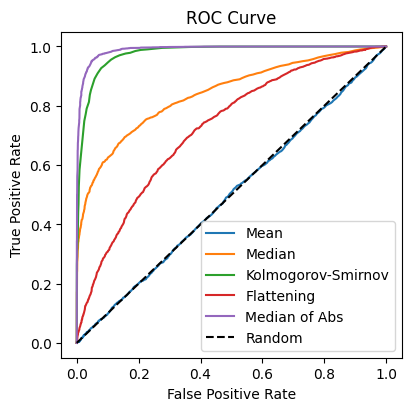
\includegraphics[width=7cm]{img/roc_curves.png}
\caption{Courbes ROC pour différentes statistiques de test sur les distribution simulées dans le contexte du VLTI avec un compagnon de contraste $10^{-2}$.}
\label{fig:roc}
\end{figure}

\begin{figure}[H]
\centering
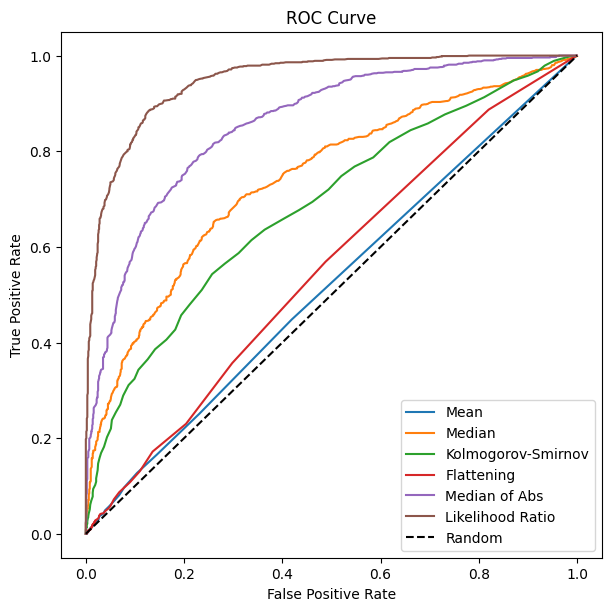
\includegraphics[width=7cm]{img/neyman_pearson.png}
\caption{Courbes ROC pour différentes statistiques de test comparées au test optimal de Neyman-Pearson, dans le contexte du VLTI avec un compagnon de contraste $10^{-3}$.}
\label{fig:neyman-pearson}
\end{figure}

\hl{Analyse des résultats}

\subsection{Analyse des valeurs P}

\dm{Attention Fig.4 c'est faux : ce ne sont pas les p-valeurs car les p-valeurs ne dépendent pas d'un seuil, seulement des données.}

Les valeurs P fournissent une mesure de confiance pour rejeter l'hypothèse nulle. Une valeur P inférieure à 0,05 est généralement considérée comme significative. \dm{Non ça ça dépend des applications. Donne la définition précise de la p-valeur tout de suite, comme ça on sait de quoi on parle. }\\

\dm{Pour l'approche Neyman-Pearson (ou Likelihood-Ratio), il faut en faire une section à part dans la section d'avant en explicitant le Likelihood-Ratio et les paramètres dont il dépend sous les 2 hypothèses, puis en tirer la stat de test que ça donne en prenant le log etc .\\
Expliquer aussi l'intérêt du NP.}.


\begin{figure}[H]
\centering
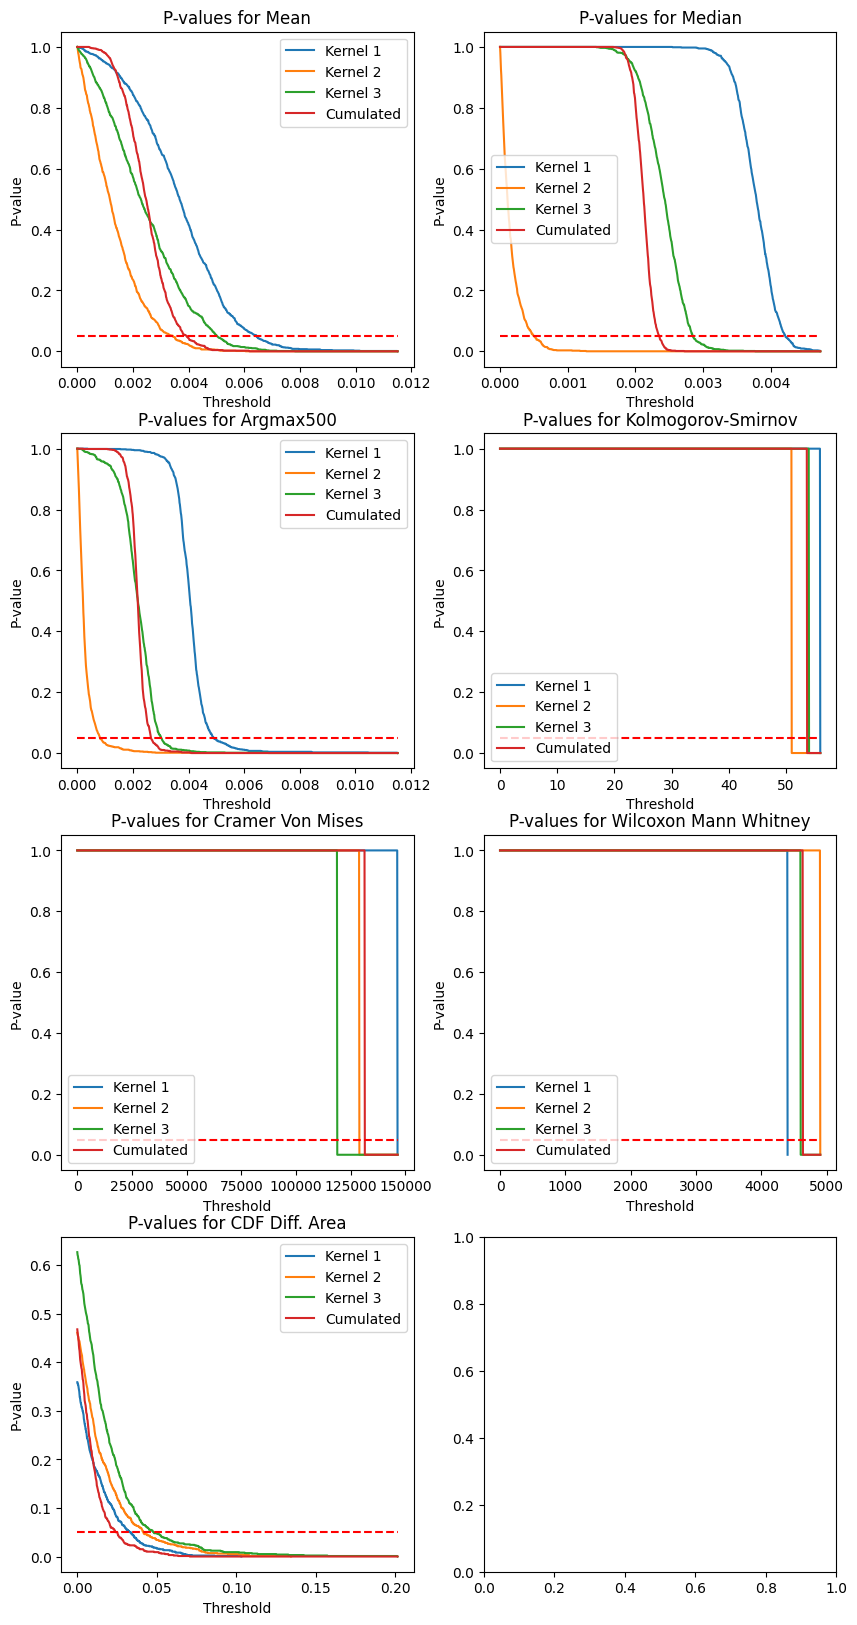
\includegraphics[width=10cm]{img/p-values.png}
\caption{Évolution des valeurs P en fonction du seuil pour différentes statistiques de test. La ligne pointillée rouge indique le seuil de significativité à 0,05. \hl{Plot à refaire pour se focaliser sur un seul Kernel (+ correction des bugs)} \dm{Oui. On peut par exemple montrer la calibration théorique p-valeur(stat de test - pas seuil !) et comparer à la calibration empirique pour chaque test }}


\label{fig:pvalues}
\end{figure}

\hl{Analyse des résultats}

%--------------------------------------------------------------------

\section{Discussion}

\subsection{Performance comparative des tests}

\hl{ToDo}

\subsection{Sensibilité au bruit}

\hl{ToDo}


%-----------------------------------------------------------------

\section{Conclusions}

\hl{ToDo}

\bibliographystyle{alpha}
\bibliography{sample}

\end{document}